\section{Durchführung}
\label{sec:Durchführung}


\subsection{Messung der Zeitkonstanten}

\sloppy
Bei dieser Messung soll die Zeitkonstante des RC-Kreises bestimmt werden. Hierzu werden ein Kondensator der Kapazität C, ein Widerstand R, 
ein Spannungsgenerator und ein Oszilloskop benötigt. Die Bauteile werden wie in \autoref{fig:schaltung1} aufgebaut. Es kann nun durch den 
Spannungsgenerator eine Rechteckspannung angelegt und die Entladekurve am Oszilloskop betrachtet werden.
\begin{figure}[H]
    \centering
    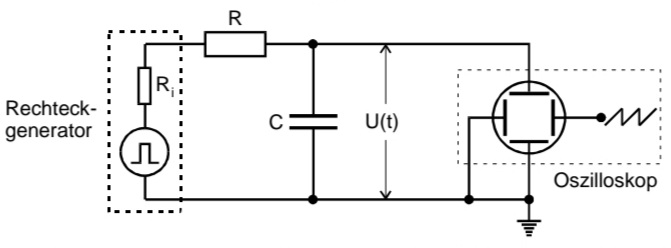
\includegraphics[width=0.75\textwidth]{Dateien/Schaltung1.jpg}
    \caption{Schaltung zur Messung der Zeitkonstante \cite{anleitung353}.}
    \label{fig:schaltung1}
\end{figure}


\subsection{Messung der Amplitude der Kondensatorspannung}
Der Versuchsaufbau bleibt bei dieser Messung unverändert zur Vorherigen. Am Spannungsgenerator wird allerdings statt der Rechtecksspannung 
eine Sinusspannung, mit einer Frequenz zwischen $\SI{50}{\hertz}$ und $\SI{60}{\kilo\hertz}$ eingestellt. Die Amplitude der 
Kondensatorspannung kann erneut am Oszilloskop abgelesen werden.


\subsection{Messung der Phasenverschiebung}

\sloppy
Der Versuchsaufbau wird anschließend so geändert, dass er dem Schaltbild auf \autoref{fig:schaltung2} entspricht. Auf dem Oszilloskop kann jeweils der Spannungsverlauf des Kondensators $U_{\text{C}}(t)$ und des
Generators $U_{\text{G}}(t)$ abgelesen werden. Es kann nun der Abstand der Nullstellen und die jeweilige Wellenlänge gemessen werden. Der Messbereich ist identisch zum Vorherigen.
\begin{figure}[H]
    \centering
    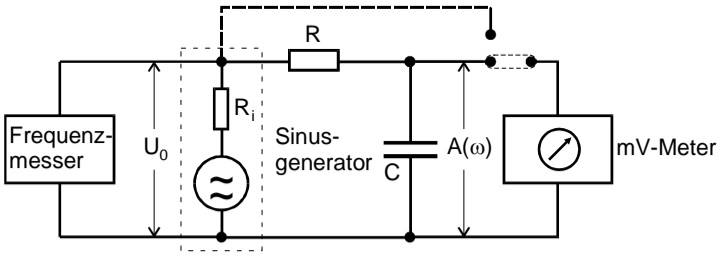
\includegraphics[width=0.75\textwidth]{Dateien/Schaltung2.jpg}
    \caption{Schaltung zur Messung der Phasenverschiebung \cite{anleitung353}.}
    \label{fig:schaltung2}
\end{figure}


\subsection{Messung zur Bestätigung der Integratorfunktion}

\sloppy
Zuletzt wird die in \autoref{fig:schaltung3} dargestellte Schaltung aufgebaut. Auf dem Zweikanal-Oszillographen sind jetzt sowohl die 
generierte, als auch die integrierte Spannung abgebildet. Am Generator werden nun nacheinander Rechtecks-, Sinus- und 
Dreiecksspannung eingestellt und jeweils das Bild des Oszillographen abfotografiert.
\begin{figure}[H]
    \centering
    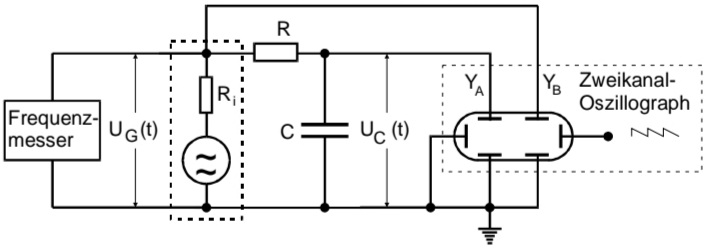
\includegraphics[width=0.75\textwidth]{Dateien/Schaltung3.jpg}
    \caption{Schaltung zur Überprüfung des Integrators \cite{anleitung353}.}
    \label{fig:schaltung3}
\end{figure}



%Aus \autoref{fig:entladekurve} ist eine Abbildung der Entladekurve auf einem Oszilloskop zu entnehmen.
%\begin{figure}[H]
%    \centering
%    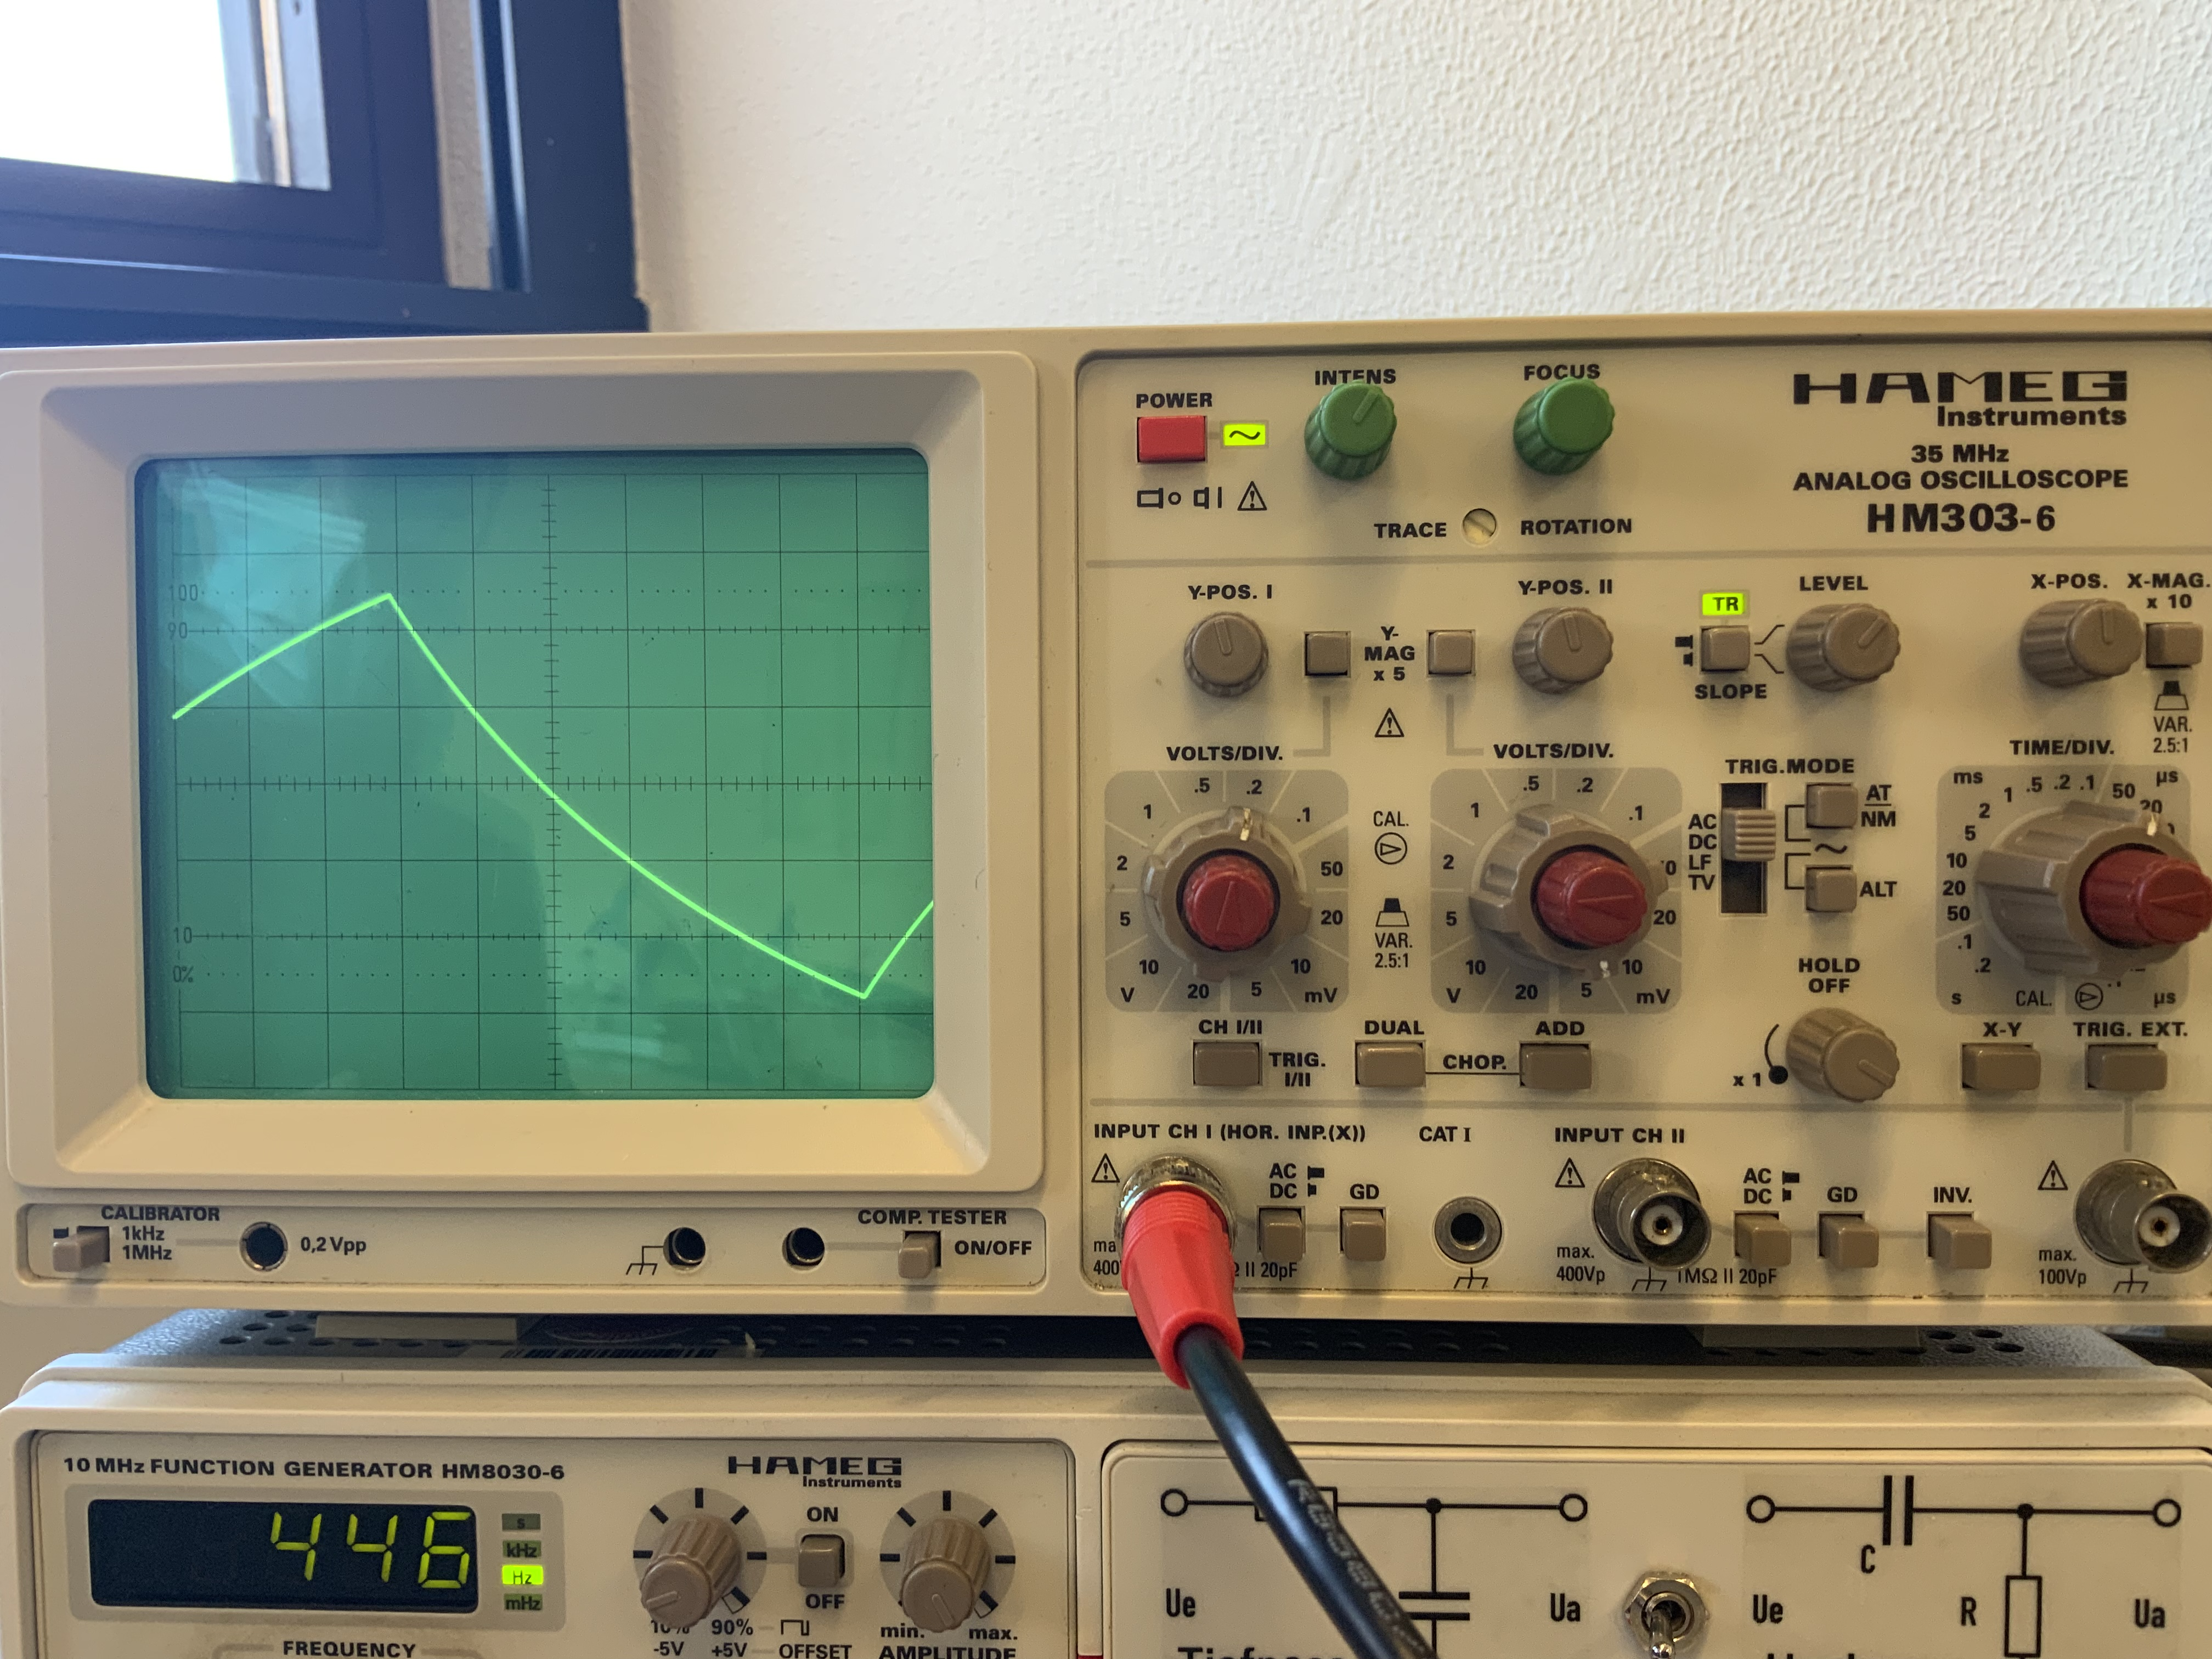
\includegraphics[width=0.75\textwidth]{Dateien/entladekurve.jpeg}
%    \caption{Entladekurve.}
%    \label{fig:entladekurve}
%\end{figure}